\documentclass{article}
\usepackage[utf8]{inputenc}
\usepackage{wrapfig}
\usepackage{graphicx}
\usepackage{float}
\graphicspath{ {images/} }
\usepackage[margin=1in]{geometry}


\title{Lógica \& realimentação proporcional}
\date{4 de Novembro de 2016}
\author{Bernardo Meurer\\
        \texttt{86242}
        \and
        Maria Adelaide Ambrósio\\
        \texttt{87064}
        \and
        Inês Coelho\\
        \texttt{87022}}
\begin{document}
\maketitle
\newpage
\section{Lógica}
\subsection{Descrição do Programa}
O programa consiste num loop destinado ao seguimento da linha preta. As
instruções dadas foram as seguintes: se o robô detetar a linha preta à direita,
a velocidade do motor esquerdo aumenta, caso contrário, se a linha preta se
encontrar à esquerda, a velocidade do motor direito aumenta. Repete este
procedimento de forma cíclica fazendo com que o robô esteja constantemente a
oscilar em torno da linha.
\begin{wrapfigure}{R}[H]
    \centering
    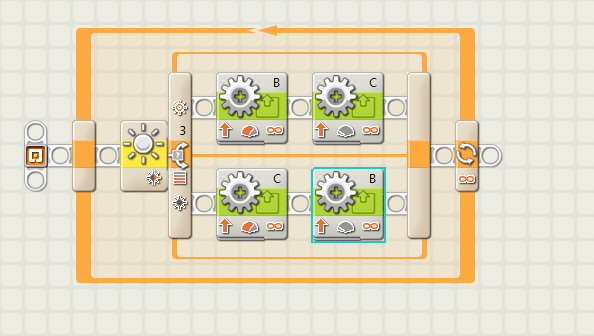
\includegraphics[scale=.5]{logica}
    \caption{Seguimento da fita baseado em lógica}
\end{wrapfigure}
\subsection{Análise das Limitações}
O nosso objetivo é fazer com que o robô siga a linha preta, efetuando o menor
número possível de mudanças de direção. Isto é, o percurso deverá ser
precisamente sobre a linha mudando de direção apenas quando a linha o faz,
fazendo com que o processo pareça o mais natural possível. Todavia, com este
tipo de programação lógica, o robô está constantemente a efetuar oscilações no
seu percurso, até mesmo quando este já se encontra sobre a linha. Assim, o
robô avança aos `s' em torno da linha o que faz com que o processo não pareça
tão natural quanto pretendíamos.

\section{Seguimento da fita baseado em Lógica com Paragem (fig.4)}
O programa consiste num loop que integra outros dois: um destinado ao seguimento
de uma linha preta (ciclo já descrito no ponto 1.1) e o outro testa se há um
obstáculo, forçando os motores a parar em caso afirmativo e a retomar a sua
marcha assim que o obstáculo seja removido. Dentro deste último existe outro
loop que faz com que o robô emita um som enquanto o obstáculo estiver no seu
caminho.
\begin{figure}[H]
    \centering
    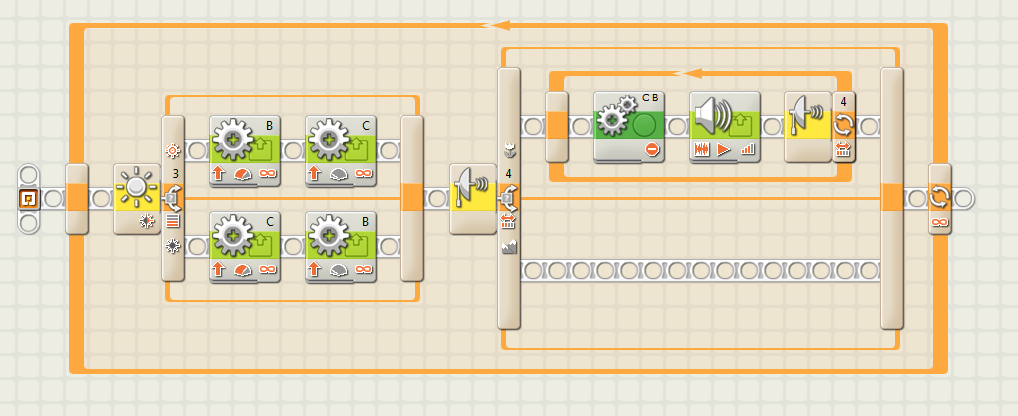
\includegraphics[scale=.5]{logica-paragem}
    \caption{Seguimento de fita com paragem}
\end{figure}

\section{Realimentação Proporcional}
\subsection{Descrição do Programa}
O programa consiste num loop infinito. Contido neste loop encontra-se a lógica
fundamental do programa. Esta consiste em obter uma leitura de luminosidade e
subtraí-la da medida de referência (neste caso 55). Consideramos esta subtração
o erro e multiplicamo-lo por um valor que controla a intensidade da resposta ao
erro, a nossa constante K (K=1,2). Ao retirmarmos este valor à velocidade que
tomamos como referência, o robô decide para que lado deve virar.
\subsection{Limitações do Programa}
Poderão haver distúrbios que os sensores não medem, logo as alterações não serão
compensadas pelo motor. Por outro lado, tem que haver conhecimento prévio das
alterações que os distúrbios provocam na variável controlada, neste caso,
 a velocidade.

\begin{figure}[H]
    \centering
    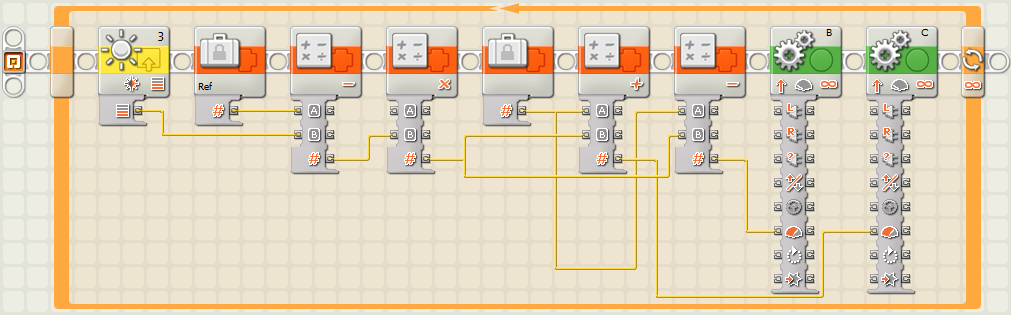
\includegraphics[scale=.5]{code}
    \caption{Seguimento da fita baseado em ralimentação proporcional}
\end{figure}

\section{Conclusão}
Nesta sessão efetuámos duas abordagens para o mesmo problema: programar um robot
capaz de seguir uma linha preta sobre um fundo branco. Utilizámos uma abordagem
baseada em lógica  e outra baseada em realimentação proporcional. Após os testes
, chegámos à conclusão que apesar da maior complexidade, o processo de
realimentação proporcional é mais eficiente.


\end{document}
